\begin{wrapfigure}[5]{r}{0.2\textwidth}
\centering
\vspace{-.6\baselineskip}
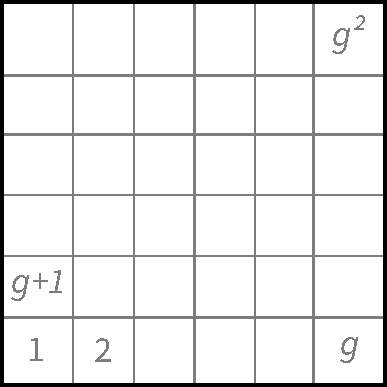
\includegraphics[width=0.15\columnwidth]{grid}
\end{wrapfigure}
Let first define some notation. As mentioned before, the city is divided in a
$g\times g$ grid made of rectangular cells $1$ through $g^2$ (like pictured on
the right). For a cell $i$, let $b(i)$ be the total number of photos in
$i$\fup{th} cell \footnote{The so called background, hence the notation.},
$B=\sum_i b(i)$ the total number of photos and $b_f(i)=\frac{b(i)}{B}$ the
frequency of each cell. For a tag $t$, we define in the same manner $t(i)$,
$T$ and $t_f(i)$, this time considering only photos which have tags $t$.

With these frequencies we can compute entropy. Let \[H(t,g) = -\frac{1}{2\log
g}\sum_{i=1}^{g^2} t_f(i)\log t_f(i)\] be the entropy of tag $t$ on a grid of
size $g$. The normalization factor ensures that regardless of $g$, the values
will range from $0$ (all photos in the same cell) to $1$ (uniform
distribution). Tags with extremal values are presented in
Table~\vref{tab:entropy} for three grids: $200\times 200$ (each cell is $80$
by $70$ meters long, less than a block), $80\times 80$ ($200\times 180$
meters, slightly more that a block) and $20\times 20$ ($800\times 700$ meters,
maybe a district). We notice that the lowest values relate to specific
location like museum while highest one are generic. Whereas $g=200$ and
$g=80$ yield comparable result, it is no more the case for $g=20$. In
particular high valued tags become even more generic (sky, dog, \dots).

\begin{table}[ht]
\centering
\setlength{\tabcolsep}{0.8em}
\begin{tabular}{lclclc}
\toprule
 \multicolumn{2}{c}{$g=200$}&  \multicolumn{2}{c}{$g=80$}&  \multicolumn{2}{c}{$g=20$}  \\
\midrule
\multicolumn{6}{c}{Lowest entropy} \\
\midrule
111minna         & .046 & theindependent         & .008 & museumofmodernart   & .002 \\
billgraham[…]    & .052 & dnalounge              & .012 & yerbabuena[…]       & .003 \\
rodin            & .053 & franklloydwright       & .022 & californiapalace[…] & .003 \\
teagarden        & .058 & greatamerican[…]       & .022 & museemecanique      & .006 \\
dnalounge        & .063 & californiapalace[…]    & .025 & cupidsspan          & .007 \\
bottomofthehill  & .064 & bottomofthehill        & .025 & pier45              & .007 \\
cafedunord       & .067 & saintspeter[…]         & .026 & missiondolorespark  & .008 \\
theindependent   & .069 & rodin                  & .034 & theindependent      & .010 \\
franklloydwright & .070 & honor                  & .035 & clarionalley        & .011 \\
warfield         & .074 & billgraham[…]          & .035 & asianartmuseum      & .012 \\
greatamerican[…] & .075 & asianartmuseum         & .038 & fairmont            & .012 \\
\midrule
\multicolumn{6}{c}{Highest entropy} \\
\midrule
usa              & .688 & color                  & .728 & sunset              & .751 \\
sf               & .696 & northerncalifornia     & .729 & dog                 & .753 \\
instagramapp     & .700 & square                 & .735 & purple              & .755 \\
square           & .700 & instagramapp           & .736 & nikon               & .756 \\
squareformat     & .700 & squareformat           & .736 & sky                 & .757 \\
iphoneography    & .703 & iphoneography          & .737 & blue                & .766 \\
unitedstates     & .703 & iphone                 & .737 & d200                & .767 \\
iphone           & .720 & california             & .738 & color               & .769 \\
foundinsf        & .724 & sanfrancisco           & .744 & northerncalifornia  & .773 \\
california       & .726 & gwsf                   & .766 & gwsf                & .812 \\
sanfrancisco     & .738 & foundinsf              & .803 & foundinsf           & .825 \\
\bottomrule
\end{tabular}
\caption{The tags with lowest and highest entropy for three different grid
	size (the abbreviated ones are \textsf{billgrahamcivicauditorium},
	\textsf{californiapalaceofthelegionofhonor},
	\textsf{yerbabuenacenterforthearts}, \textsf{greatamericanmusichall} and
\textsf{saintspeterandpaulchurch}).\label{tab:entropy}}
\end{table}

To further differentiate tags that are highly concentrated, we can compute the
Kullback Leibler divergence of their distribution with the one of all the
photos. For that, we define \[D_g(t||b) = \frac{-1}{\log
	\min_{b_f(i)>0}b_f(i)}\sum_{i=1,\, b_f(i)>0}^{g^2} t_f(i)\log
\frac{t_f(i)}{b_f(i)}\] This time, values range from $1$ (when all the $t$
photos are in the cell where there are the fewest total photos and thus are
maximally distinct) to $0$ (for $t=b$, which is not possible). Again extremal
values are shown in Table~\vref{tab:kl}. It also differentiates between the
two kinds of tag but compared with entropy, it seems more robust to change in
the grid dimensions as the three rows shows roughly the same set of tags.
Weirdly enough, there is also a semantic shift for position specific tags.
Whereas those picked by entropy were mostly buildings, here they relate more to
recreational areas like parks.

\begin{table}[ht]
\centering
\setlength{\tabcolsep}{1.2em}
\begin{tabular}{lclclc}
\toprule
 \multicolumn{2}{c}{$g=200$}&  \multicolumn{2}{c}{$g=80$}&  \multicolumn{2}{c}{$g=20$}  \\
\midrule
\multicolumn{6}{c}{Highest divergence} \\
\midrule
lakemerced     & .587 & lakemerced      & .568 & grandviewpark   & .506 \\
grandviewpark  & .563 & grandviewpark   & .554 & lakemerced      & .485 \\
hunterspoint   & .533 & hunterspoint    & .520 & sterngrove      & .484 \\
sterngrove     & .532 & westportal      & .514 & hunterspoint    & .477 \\
westportal     & .528 & sterngrove      & .512 & fortfunston     & .459 \\
catamaran      & .524 & chinabeach      & .502 & chinabeach      & .450 \\
dubocepark     & .519 & dubocepark      & .484 & westportal      & .446 \\
buenavistapark & .518 & glenpark        & .482 & nfl             & .441 \\
chinabeach     & .518 & buenavistapark  & .477 & candlestickpark & .440 \\
ccsf           & .517 & candlestickpark & .477 & glenpark        & .432 \\
glenpark       & .508 & fortfunston     & .471 & sfsu            & .430 \\
\midrule
\multicolumn{6}{c}{Lowest divergence} \\
\midrule
san           & .058 & san           & .032 & squareformat  & .011 \\
ca            & .058 & ca            & .030 & 2011          & .011 \\
instagramapp  & .055 & instagramapp  & .030 & square        & .011 \\
squareformat  & .055 & squareformat  & .030 & iphoneography & .011 \\
square        & .054 & unitedstates  & .030 & francisco     & .010 \\
iphoneography & .053 & square        & .030 & san           & .010 \\
unitedstates  & .053 & iphoneography & .029 & unitedstates  & .009 \\
usa           & .046 & usa           & .026 & ca            & .008 \\
sf            & .042 & sf            & .021 & sf            & .006 \\
california    & .021 & california    & .011 & california    & .004 \\
sanfrancisco  & .011 & sanfrancisco  & .006 & sanfrancisco  & .002 \\
\bottomrule
\end{tabular}
\caption{The tags with lowest and highest Kullback Leibler divergence for
	three different grid size.\label{tab:kl}}
\end{table}

This two statistics are interesting but they have one major drawback, they
give a single value for each tag. While this is convenient for ranking them,
it loses all the information about their position. That why we finally use the
Kulldorf spatial scan statistic\cite{kulldorff}. Let $R_{i,w,h}$ be a
rectangular region defined by its bottom left cell $i$, its width $w$ and its
height $h$ as the following set of cells: \[R_{i,w,h} = \{i + k + lg,\,
k\in\llbracket 0,\dots, w-1\rrbracket,\, l\in\llbracket 0,\dots,
h-1\rrbracket\}\] For a given $R$, what we will now call its discrepancy with
respect to tag $t$ is
\[
	d(t, R) =
\begin{dcases}
	t_f(R)\log\frac{t_f(R)}{b_f(R)} + (1-t_f(R))\log\frac{1-t_f(R)}{1-b_f(R)}
	& \text{if } \frac{t_f}{b_f} \geq \frac{1-t_f}{1-b_f} \text{ and } t_f \geq T\\
	0 & \text{otherwise}
\end{dcases}
\]
and we recognize the Kullback Leibler divergence restricted to $R$ and its
complementary. $T$ is a threshold ensuring that we consider only region with
enough support to be significant.

To compute it, we implemented the exhaustive method described in
\citep[Algorithm 3]{Agarwal2006spatial} with two modifications. First, letting
$w$ and $h$ go from $1$ to $g$, there are $g^2\cdot g\cdot g$ possible
regions. But to speed up computations and because we did not want to get
regions covering a large portion of the city, we restricted their maximum
size. Then, instead of returning the most discrepant region, we maintained a
list of the top $K$ ones. Like before, it is informative to look at
Table~\vref{t:disc} to see which tags get high and low values (over all their
regions). This time, the values are not normalized between different grid size
hence only the relative order is meaningfull. Again tag with high discrepancy
are related with locations such as parks. On the other side, tags with low
discrepancy are more difficult to interpret because they mostly do not refer
to geographic features.

\begin{table}[ht]
\centering
\setlength{\tabcolsep}{1.2em}
\begin{tabular}{lclclc}
\toprule
 \multicolumn{2}{c}{$g=200$}&  \multicolumn{2}{c}{$g=80$}&  \multicolumn{2}{c}{$g=20$}  \\
\midrule
\multicolumn{6}{c}{Highest discrepancy} \\
\midrule
grandviewpark     & 7.493 & grandviewpark   & 7.113 & grandviewpark       & 6.521 \\
sterngrove        & 7.208 & sterngrove      & 6.338 & sterngrove          & 5.998 \\
local             & 6.881 & candlestickpark & 6.318 & fortfunston         & 5.924 \\
alcohol           & 6.666 & dubocepark      & 6.152 & candlestickpark     & 5.638 \\
dubocepark        & 6.467 & pier7           & 6.072 & bayareadisco[…]     & 5.484 \\
yoda              & 6.467 & nfl             & 6.052 & nfl                 & 5.411 \\
coronaheights     & 6.374 & fortfunston     & 5.948 & chinabeach          & 5.392 \\
performer         & 6.374 & bottomofthehill & 5.917 & glenpark            & 5.338 \\
circus            & 6.371 & slims           & 5.804 & sfsu                & 5.326 \\
candlestickpark   & 6.285 & westportal      & 5.752 & westportal          & 5.258 \\
bernalheightspark & 6.158 & bayareadisco[…] & 5.732 & californiapalace[…] & 5.225 \\
\midrule
\multicolumn{6}{c}{Lowest discrepancy} \\
\midrule
instagramapp  & 0.013 & street      & 0.062 & logo        & 0.054 \\
squareformat  & 0.013 & sign        & 0.062 & friends     & 0.053 \\
square        & 0.012 & lofi        & 0.061 & sign        & 0.053 \\
iphoneography & 0.012 & hair        & 0.059 & yellow      & 0.052 \\
sf            & 0.009 & hipstamatic & 0.059 & bayarea     & 0.051 \\
xproii        & 0.008 & food        & 0.059 & shozu       & 0.051 \\
sierra        & 0.007 & motionblur  & 0.057 & party       & 0.050 \\
california    & 0.004 & large       & 0.056 & mirror      & 0.050 \\
rise          & 0.003 & 2009        & 0.056 & hipstamatic & 0.050 \\
amaro         & 0.002 & nashville   & 0.056 & purple      & 0.049 \\
sanfrancisco  & 0.001 & bayarea     & 0.055 & truck       & 0.048 \\
\bottomrule
\end{tabular}
\caption{Tags with lowest and highest discrepancy for three different grid
size (the abbreviated ones are \textsf{bayareadiscorymuseum} and
	\textsf{californiapalaceofthelegionofhonor}).\label{t:disc}}
\end{table}
